% ------------------------------------------------------------------------
% ------------------------------------------------------------------------
% ------------------------------------------------------------------------
%                                Capítulo 4
% ------------------------------------------------------------------------
% ------------------------------------------------------------------------
% ------------------------------------------------------------------------
%https://programmerclick.com/article/61381626434/
%\chapter{RELAJACIÓN ESTRUCTURAL DE LAS CONFIGURACIONES RP ENCONTRADAS}
% ------------------------------------------------------------------------.
\section{RELAJACIÓN ESTRUCTURAL DE LAS CONFIGURACIONES RP}\label{Sec. 2.2}

La relajación estructural, o también conocida como optimización, es un cálculo necesario para ajustar los sitios cristalográficos y así minimizar la energía interna de la estructura. Es decir, el cálculo desplaza los iones hasta que las fuerzas interatómicas sean casi nulas ($\sim0.02 eV$) y llegar a un estado estable. En esta sección se discuten los detalles computacionales mas relevante para el cálculo, como el parámetro de Hubbard \textsc{u} que corrige el sitio de Coulomb; además se discuten los detalles estructurales de cada configuración, como los parámetros de red, la energía de la estructura y sus cambios debido a la relajación.

\subsection{Relevantes detalles computacionales: Parámetro de Hubbard \textsc{u}}

La optimización estructural de \textsc{rp} $Sr_{2}(Ta,Nb)O_{3-x}N_{x}$(x=0.5 y 1.0) fue realizada mediante cálculos de primeros principios, con base en la teoría funcional de la densidad (\textsc{dft}) implementada en el código \textsc{vasp}\cite{urlvasp}. Se usó \textsc{vasp} debido a la alta precisión que tienen los pseudopotenciales basados en ondas planas \textsc{'paw'}, por sus siglas \textbf{P}lane \textbf{A}ugmented \textbf{W}aves. Los pseudopotenciales usados fueron \textsc{pbe}\textit{sol} dentro de la aproximación del funcional de intercambio-correlación \textsc{gga+u}. Es necesario introducir el parámetro \textsc{'u'} a los elementos que son altamente correlacionados ($3d$, $4d$, $5d$, magnéticos) como lo son los metales de transición niobio ($Nb$) y Tántalo ($Ta$), esto corrige la correlación a través de introducir un termino adicional en el hamiltoniano. El término de la corrección de Hubbard \textsc{'u'} entra como una energía en los orbitales, corrige la fuerza de las interacciones en el sitio de Coulomb, corrige los orbitales y la separación entre ellos (Liechtenstein\cite{Lichtenstein1995StrongOrdering}).

Los sistemas correlacionados están mal descritos por los cálculos de \textsc{dft}\cite{Tolba2018}, la manera estándar como calcula la energía no es suficiente, así que el parámetro \textsc{u} corrige la energía de correlación. A menudo, el valor \textsc{u} no se conoce y prácticamente se modifica semi-empíricamente para hacer buenos resultados computacionales en base a datos experimentales. En la literatura se encuentran varios ejemplos que muestran la relación entre el parámetro \textsc{u} y las propiedades físicas predichas:

\begin{itemize}
    \item En el estudio teórico del material $M_{3}O_{4}(M=V, Cr, Mn, Fe, Co, Ni, Cu)$ hecho por Wang et. al. \cite{Wang2006} identifican dos contribuciones al error en las energías de oxidación cuando usan el enfoque \textsc{gga}: La primera contribución se origina en la sobre-estimación del enlace en la molécula de $O_{2}$; el segundo error está relacionado con el error de correlación en orbitales $3d$,  lo que resulta en una sobre-estimación de las energías de oxidación. El enfoque \textsc{gga+u} elimina el error del enlace de $O_{2}$, permitiendo abordar los efectos de correlación en los metales de transición $3d$. Se han utilizado una variedad de valores de \textsc{u} que van de $2$ a $6 eV$ para las propiedades, incluidas la estructura de bandas, la energía de oxidación y los parámetros estructurales \cite{Wang2006}.% La banda prohibida calculada en la aproximación de gradiente generalizada (GGA) + U concuerda bien con el valor experimental de 1,6 eV. Por otro lado, el valor calculado utilizando el híbrido funcional PBE0 (3,42 eV) está muy sobreestimado, debido a que se descuida el problema de apantallamineto de la aproximación de Hartree-Fock [25]. 
    \item En materiales con metales orgánicos (\textsc{mof}), por sus siglas en inglés '\textsc{M}etal \textsc{O}rganics \textsc{F}ramework', investigado por Mann et. al. \cite{Mann2016}, muestran que la energía de enlace de $MO_{2}$ en $M-MOF-74 (M=Ti,V,Cr,Mn,Fe,Co,Ni,Cu)$ crece linealmente con el valor de Hubbard \textsc{u}, se desplaza $0,041  eV$ sobre el rango de $U = 0-5,4  eV$. Para el caso del cobalto $Co$, los parámetros de red coinciden con el experimento por el hecho de que la longitud del enlace $Co-O$ disminuye con \textsc{u}, el parámetro localiza los estados $d$ de $Co$ lo que permite que la molécula de $CoO_{2}$ se acerque más al sitio del \textsc{mof}, aumentando la contribución electrostática a la energía de enlace \cite{Mann2016}.
     
    \item Dentro del estudio de $BiMnO_{3}$ realizado por Boukhvalov et. al. \cite{Boukhvalov2010} señalan la desestimación de \textsc{gga} en las distorsiones Jahn-Teller. Como los octaedros $MnO_{6}$ tiene distorsiones fuertes, utilizan la teoría funcional de la densidad con la corrección de Coulomb \textsc{dft+u}. El estudio mostró que un valor de $U=2 eV$ hace que los resultados se aproximen a los datos experimentales. Además, para valores grandes de \textsc{u} ($4$ y $8 eV$) disminuye la hibridación $3d-2p$, por ende, incrementa la distancia del enlace $Mn-O$ disminuyendo los efectos de enlace. \cite{Boukhvalov2010}.
    
    \item La \href{https://pubs.acs.org/doi/suppl/10.1021/acsmaterialslett.9b00088/suppl_file/tz9b00088_si_001.pdf}{información suplementaria} del trabajo de Ouhbi y Ulrich \cite{Ulrich2019} muestra la evolución de la densidad de estados con el aumento del parámetro \textsc{u}. Se observa un cambio significativo a partir de $U=4  eV$ para el material $SrTaO_{2}N$, además de reportar cambios en la brecha entre la banda de valencia y la banda de conducción de la estructura de bandas electrónica.
\end{itemize}

%\textsc{dft+u} ha demostrados ser simple en términos de formulación teórica e implementación practica con un considerable bajo costo computacional\cite{Tolba2018}. 
En general, cuanto más localizado es un sistema, más sensible es al valor de \textsc{u} \cite{Tolba2018}. En el caso de esta investigación, la corrección se realiza para el niobio $Nb$ y el tántalo $Ta$ con un valor de $U=4.0 eV$. La comparación entre la relajación estructural usando \textsc{dft} y \textsc{dft+u} se presenta en el anexo \ref{anexoB}. Además, se agregó la energía de corte que controla el numero de ondas planas (\textsc{paw}), con un valor de $550 eV$; en la malla de puntos $k$ de la zona de Brillouin se aplica el método Monkhorst-Pack \cite{Monkh1976} para discretizar el espacio y conocer el numero de puntos que definen correctamente el sistema, en este caso se uso una malla de $8\times8\times4$. 
 
Esta sección empieza con el análisis composicional de las estructuras oxinitradas, luego se abordara el análisis energético de cada configuración para dos tipos de concentración de nitrógeno: $x=0.5$ y $x=1.0$.

\subsection{Diagrama de concentraciones aniónicas}

En un diagrama de concentraciones aniónicas, ó convex hull, se involucra la diferencia de energía respecto a las estructuras puras en función de las concentraciones aniónicas $x=0.0$, $x=0.5$, $x=1.0$ y $x=4.0$, como se muestra en la figura \ref{Fig. concentraciones-totales}. Las estructuras puras de óxido $Sr_{2}(Ta,Nb)O_{4}$ y nitruros $Sr_{2}(Ta,Nb)N_{4}$ son usadas como referencia para comparar la energía de las concentraciones $x=0.5$ y $x=1.0$.

\begin{figure}[H]
    \centering
    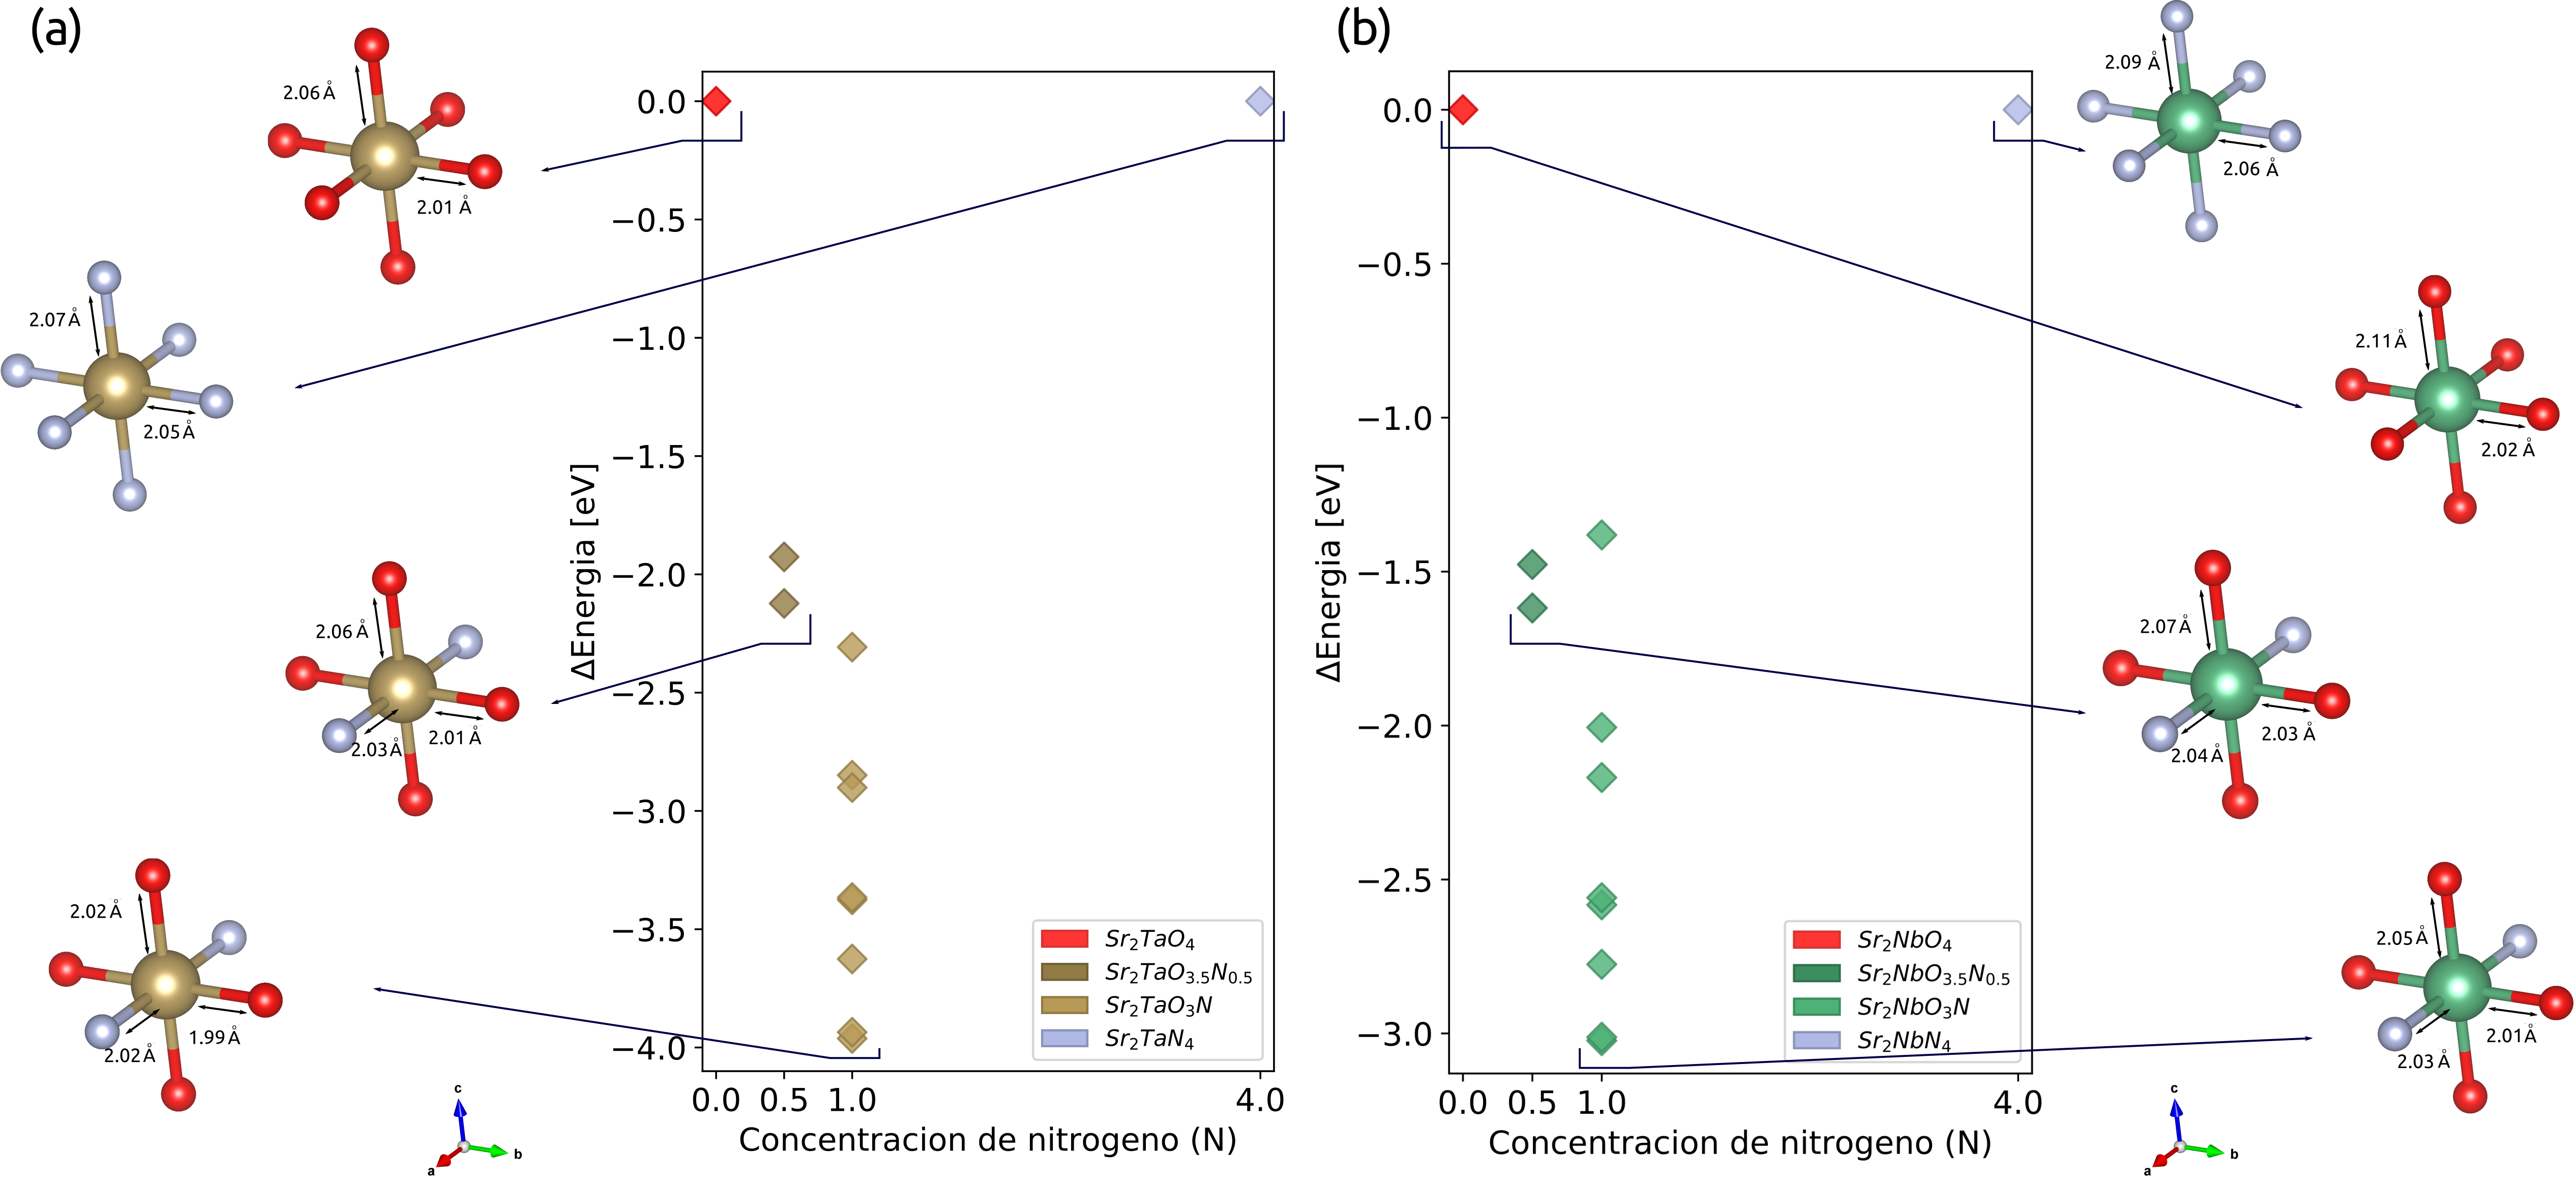
\includegraphics[width=\textwidth]{Figs/convex_hull.png}
    \caption{Diagrama de concentraciones de oxígeno y nitrógeno para $x=0.5$ y $x=1.0$ en las estructuras cristalinas Ruddlesden-Popper (a) $Sr_{2}TaO_{4-x}N_{x}$ y (b) $Sr_{2}NbO_{4-x}N_{x}$.}
    \label{Fig. concentraciones-totales}
\end{figure}

En cada concentración las configuraciones mas favorables son las de menor energía. Al observar la concentración $x=0.5$ se encuentra la configuración mas favorable en $-2.12 eV$ y $-1.62 eV$ para $Sr_{2}TaO_{3.5}N_{0.5}$ y $Sr_{2}NbO_{3.5}N_{0.5}$ respectivamente. En la concentración $x=1.0$ se encuentra la configuración mas favorable en $-3.96 eV$ y $-3.02 eV$ para $Sr_{2}TaO_{3}N$ y $Sr_{2}NbO_{3}N$ respectivamente. Las configuraciones inestables siempre aparecerán por encima de las configuraciones favorables. Las configuraciones con concentración x=1.0 son mas estables comparadas con las configuraciones con concentración x=0.5 debido a un mayor contenido de nitrógeno en la estructura, mostrando que el nitrógeno si reduce las energía estructural comparada con los oxidos y los nitruros puros.

La distancia de los enlaces $(Ta,Nb)-O$ y $(Ta,Nb)-N$ se mantienen para ambos compuestos, entre $2.02  \si{\angstrom}$ y $2.07  \si{\angstrom}$ como se reporta experimentalmente \cite{Diot1999CrystalN,Tobias2004,Clarke2002,Ebbinghaus2004PowderK,Tobias2010ChemInform2.}. Las distancias son muy similares ya que el nitrógeno tiene un radio iónico ligeramente mayor en comparación con el oxigeno, pero esto es compensado con un acortamiento del enlace asociado a una mayor covalencia con el metal de transición \cite{Yang2011,Ebbinghaus2004PowderK}.  El efecto combinado de los enlaces $(Ta,Nb)-O$ y $(Ta,Nb)-N$ y la distribución no uniforme de $N/O$ rompen la simetría del cristal, por lo que es común que las estructuras oxinitradas caigan a una simetría mas baja que $I4/mmm(139)$. Para continuar con el análisis, la siguiente sección presenta el acoplamiento entre la energía estructural de cada configuración y los ordenamientos aniónicos obtenidos en la substitución aniónica.

%. P. Ong, L. Wang, B. Kang, G. Ceder., The Li-Fe-P-O2 Phase Diagram from First Principles Calculations, Chemistry of Materials, vol. 20, Mar. 2008, pp. 1798-1807.
%S.P. Ong, A. Jain, G. Hautier, B. Kang, and G. Ceder, Thermal stabilities of delithiated olivine MPO4 (M=Fe, Mn) cathodes investigated using first principles calculations, Electrochemistry Communications, vol. 12, 2010, pp. 427-430.
 
%[REF: Vaadium oxynitrides as stable catalysts...(Pan)]
 
\subsection{Energía de las configuraciones $Sr_{2}(Ta,Nb)O_{3.5}N_{0.5}$}

La sustitución aniónica x=0.5 resultó en dos configuraciones con diferente ordenamiento aniónico. La energía estructural de cada configuración se muestra en la figura \ref{Fig. 35u-rp}.

\begin{figure}[H]
    \centering
    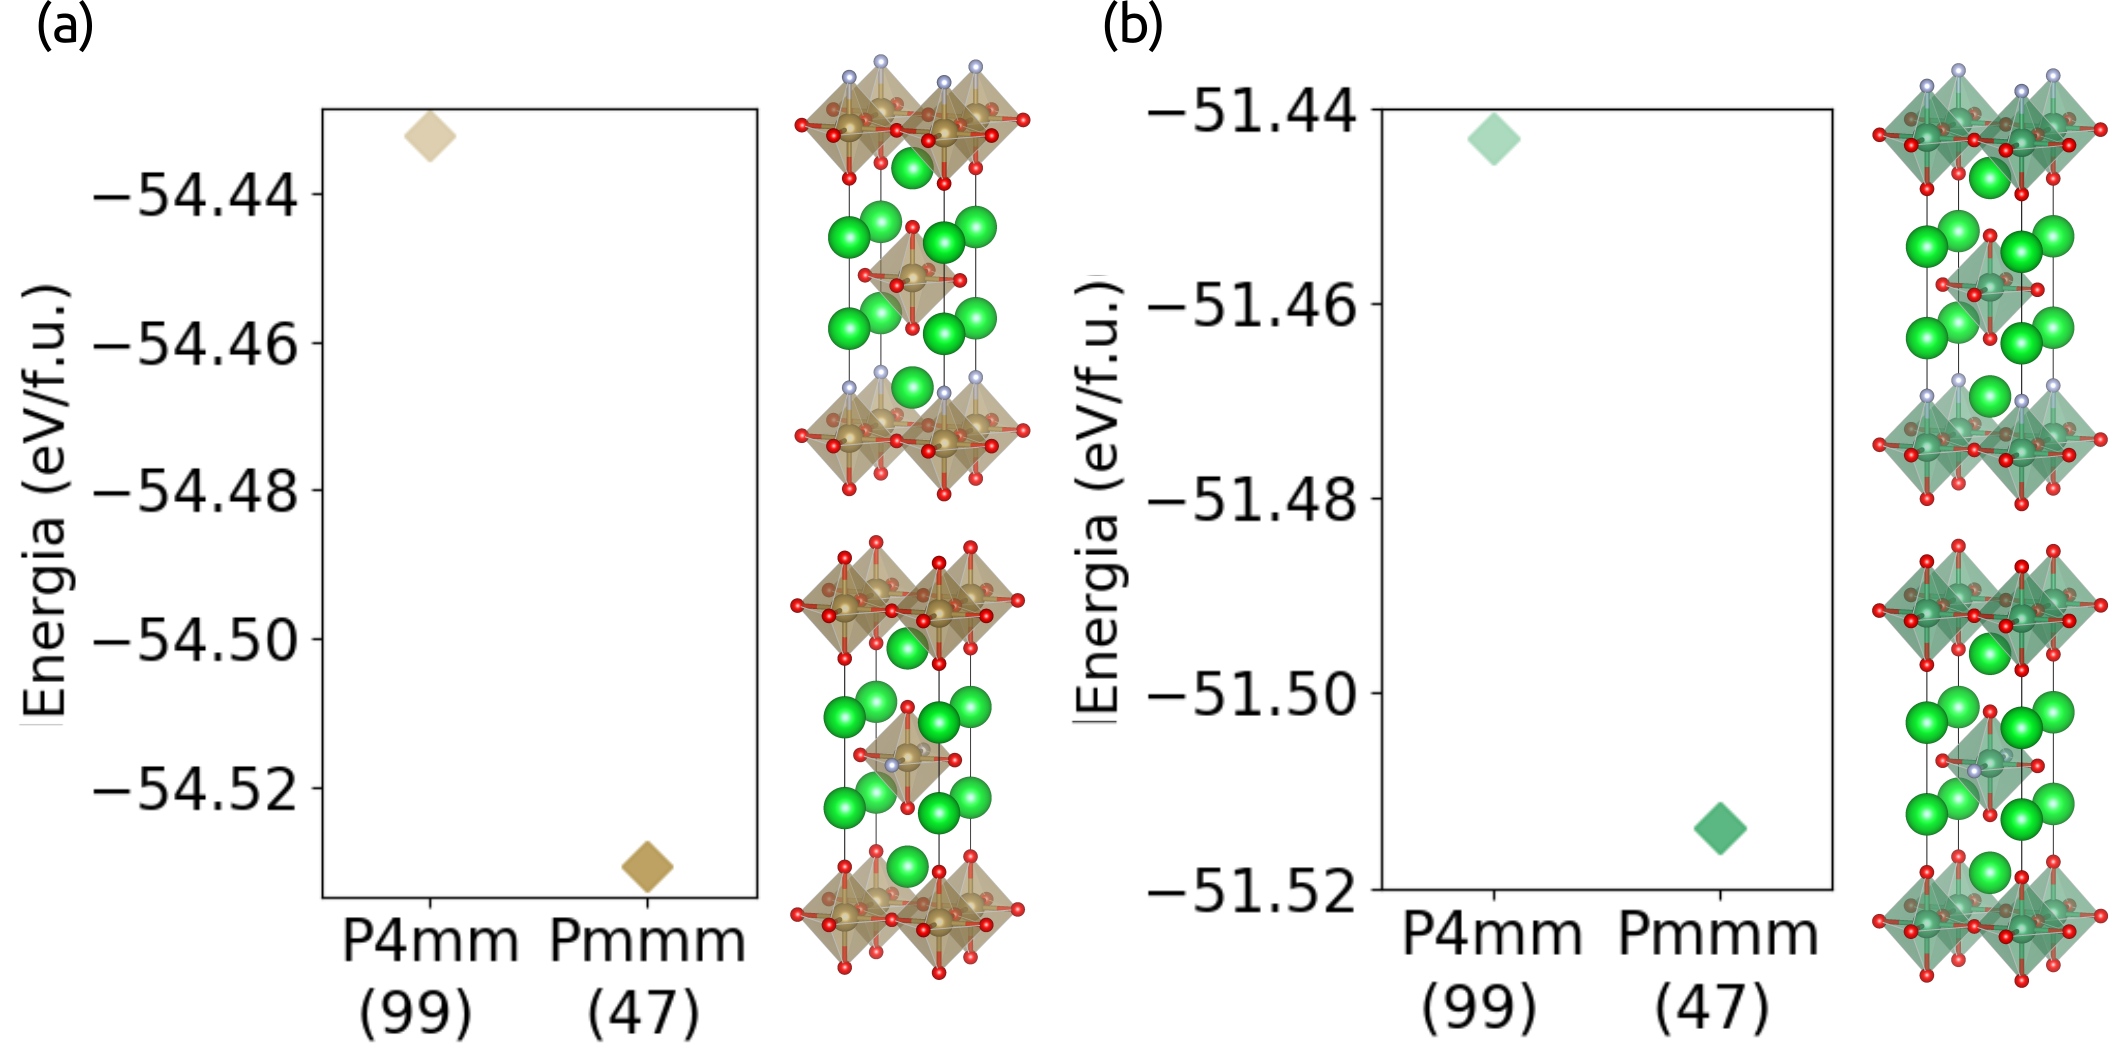
\includegraphics[width=\textwidth]{Figs/35u-rp.png}
    \caption{Energía estructural de la concentración $x=0.5$ en función del grupo de simetría espacial para las configuraciones \textsc{rp} (a) $Sr_{2}TaO_{3.5}N_{0.5}$ y (b) $Sr_{2}NbO_{3.5}N_{0.5}$.}
    \label{Fig. 35u-rp}
\end{figure}

Las estructuras de mínima energía tienen simetría de grupo espacial $Pmmm(47)$ con un valor de $-54.53 eV$ y $-51.51  eV$ respectivamente. Esta configuración favorable exhibe un ordenamiento aniónico \emph{trans} en el octaedro central, pero los octaedros de las esquinas contienen únicamente oxígeno. Esto es debido al poco contenido de nitrógeno introducido en las estructuras, el nitrógeno se sitúa en un solo sitio cristalográfico que, por simetría, se situó en el sitio ecuatorial de manera \emph{trans}. Igualmente pasa con la configuración $P4mm(99)$, el nitrógeno se ubica en el sitio superior del octaedro. La energía de la configuración \emph{trans-}$47$ indica que los nitrógenos prefieren situarse en sitios ecuatoriales que en sitios axiales del octaedro.

Los parámetros de red de la configuración ($47$)-$Sr_{2}TaO_{3.5}N_{0.5}$ son $a=4.06508 \si{\angstrom}$, $b=4.03416 \si{\angstrom}$ y $c=12.56372 \si{\angstrom}$, $\alpha=\beta=\gamma=90^{\circ}$, y volumen $206.034796 \left[\si{\angstrom}^{3}\right]$,  lo parámetros de red de la configuración ($47$)-$Sr_{2}NbO_{3.5}N_{0.5}$ son $a=4.09052$, $b=4.07287 \si{\angstrom}$ y $c=12.56518 \si{\angstrom}$, $\alpha=\beta=\gamma=90^{\circ}$, y volumen $209.337701  \si{\angstrom}^{3}$. Comparando estos parámetro de red con las estructuras de óxidos puros, el parámetro en \emph{'a'} aumenta $\sim0.04  \si{\angstrom}$, mientras que en la dirección \emph{'c'} el parámetro de red disminuye $\sim0.1 \si{\angstrom}$.

\subsection{Energía de las configuraciones $Sr_{2}(Ta,Nb)O_{3}N$}

La sustitución aniónica x=1.0 resultó en ocho configuraciones con diferente ordenamiento aniónico. La energía estructural de cada configuración se muestra en la figura \ref{Fig. rp_ta-nb_energy}.

\begin{figure}[H]
    \centering
    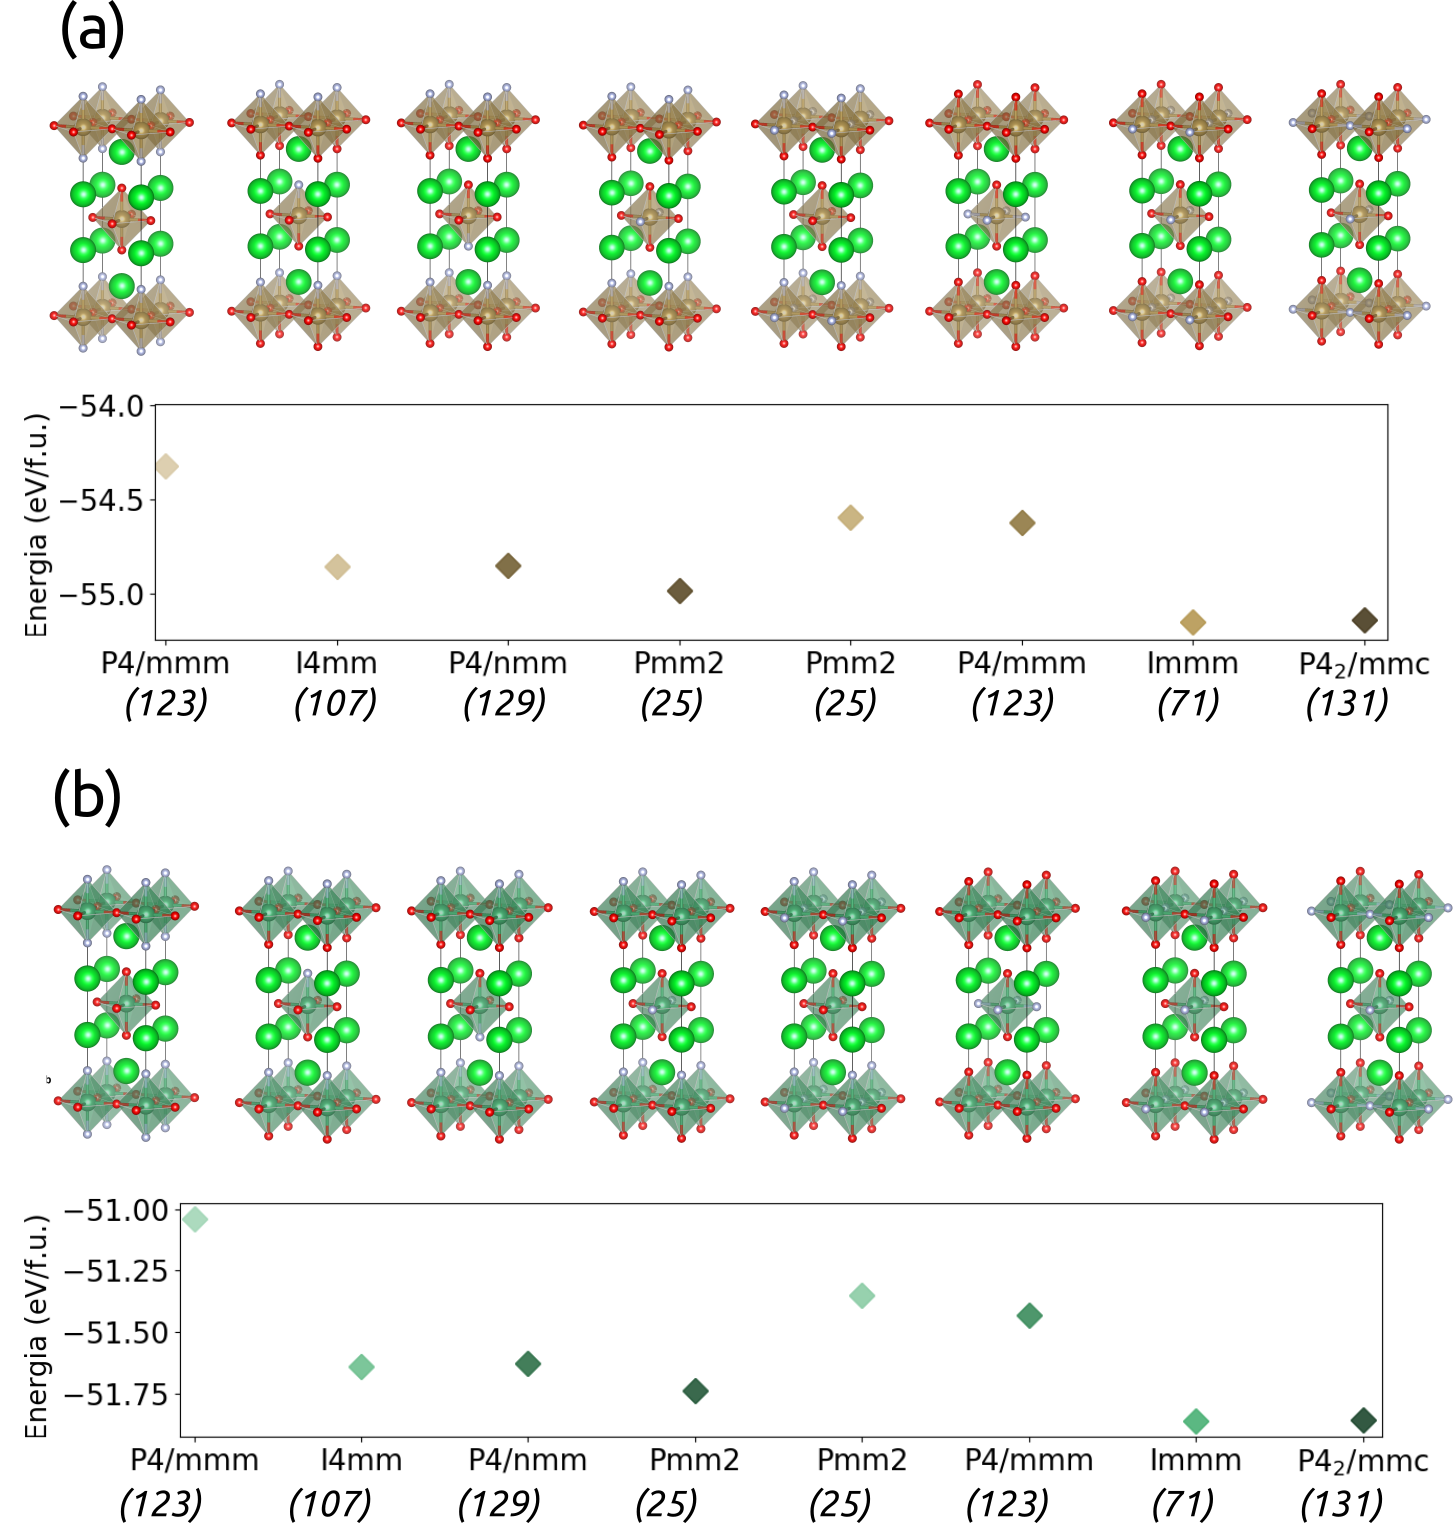
\includegraphics[width=\textwidth]{Figs/rp_ta--nb_U.png}
    \caption{Energía estructural de la concentración $x=1.0$ en función del grupo de simetría espacial para las configuraciones \textsc{rp} (a) $Sr_{2}TaO_{3}N$ y (b) $Sr_{2}NbO_{3}N$.}
    \label{Fig. rp_ta-nb_energy}
\end{figure}

Las configuraciones menos favorable están en el rango de $-54.25 eV$ a $-54.75 eV$, y $-51.00 eV$ a $-51.50 eV$ para $Sr_{2}TaO_{3}N$ y  $Sr_{2}NbO_{3}N$, respectivamente. En este rango hay tres configuraciones con grupo espacial (123), (25), (123), y presentan la particularidad de que son configuraciones donde no hay nitrógeno en algún octaedro, es decir el nitrógeno se alterna capa a capa en la perovskita \textsc{rp}, alcanzando energías iguales a las configuraciones $Sr_{2}(Ta,Nb)O_{3.5}N_{0.5}$. Esto indica que el nitrógeno debe ocupar todos los octaedros de la celda unitaria para lograr una menor energía. Las configuraciones no tan favorables están en el rango de $-54.27$ a $-55.00 eV$, y $-51.50 eV$ a $-51.75 eV$ para $Sr_{2}TaO_{3}N$ y  $Sr_{2}NbO_{3}N$, respectivamente. En este rango hay tres configuraciones con grupo espacial (107), (129), (25), presentan orden de aniones axial en todos sus octaedros. La configuración de mínima energía tienen simetría de grupo espacial $Immm(71)$ con un valor de $-55.15  eV$ y $-51.86  eV$ para $Sr_{2}TaO_{3}N$ y  $Sr_{2}NbO_{3}N$,s respectivamente. Esta configuración favorable exhibe un ordenamiento aniónico \emph{trans} con dirección \emph{'a'} en sus octaedros, todos sobre el sitio ecuatorial. La configuración $P4_{2}/mmc(131)$ también exhibe ordenamiento \emph{trans}, unas capas en dirección \emph{'a'} y otras capas en dirección \emph{'b'}, lo que la diferencia con la configuración $(71)$. Los parámetros de red de la configuración ($71$)-$Sr_{2}TaO_{3}N$ son $a=4.07855 \si{\angstrom}$, $b=4.01907 \si{\angstrom}$ y $c=12.60903 \si{\angstrom}$, $\alpha=\beta=\gamma=90^{\circ}$, y volumen $206.687252\si{\angstrom}^{3}$,  lo parámetros de red de la configuración ($71$)-$Sr_{2}NbO_{3}N$ son $a=4.08308$, $b=4.05652 \si{\angstrom}$ y $c=12.62466 \si{\angstrom}$, $\alpha=\beta=\gamma=90^{\circ}$, y volumen $209.1035  \si{\angstrom}^{3}$. Comparando estos parámetro de red con las estructuras de óxidos puros, el parámetro en \emph{'a'} aumenta $\sim0.04  \si{\angstrom}$, siendo esta la dirección del enlace $(Ta,Nb)-N$, es decir la dirección del orden aniónico \emph{trans}, mientras que en la dirección \emph{'b'}, el parámetro de red disminuye $\sim0.01 \si{\angstrom}$.

Se observa que las configuraciones mas favorables tienen ordenamiento aniónico \emph{trans}, tanto para la estructura oxinitrada \textsc{rp-}$Sr_{2}(Ta,Nb)O_{3}N$ como para  \textsc{rp-}$Sr_{2}(Ta,Nb)O_{3.5}N_{0.5}$. La conectividad de los aniones ecuatoriales requiere que cada anión esté vinculado a dos sitios del metal de transición \cite{Harada2019}, lo que solo deja dos ordenamientos posibles: \emph{cis} y \emph{trans}. Aunque en el estudio no se encontró orden de aniones \emph{cis}, y debido a los reportes experimentales y computacionales sobre una posible configuración favorable en oxinitruros con ordenamiento aniónico \emph{cis} \cite{Masubuchi2013SynthesisCeramics,Yang2011,Harada2019, Bouri2018}, es necesario buscar este ordenamiento en una celda unitaria mas grande.

\subsection{Caso especial: Configuración \emph{cis} con concentración x=1.0}

Para el estudio de la configuración \emph{cis}, se crea una supercelda con una rotación de $45^{\circ}$. Se obtuvieron 3 configuraciones con ordenamiento \emph{cis} en el plano para la concentración $x=1.0$ en ambos compuestos. La energía estructural de cada una de estas configuraciones se muestra en la figura \ref{Fig. rp_cis}.

\begin{figure}[H]
    \centering
    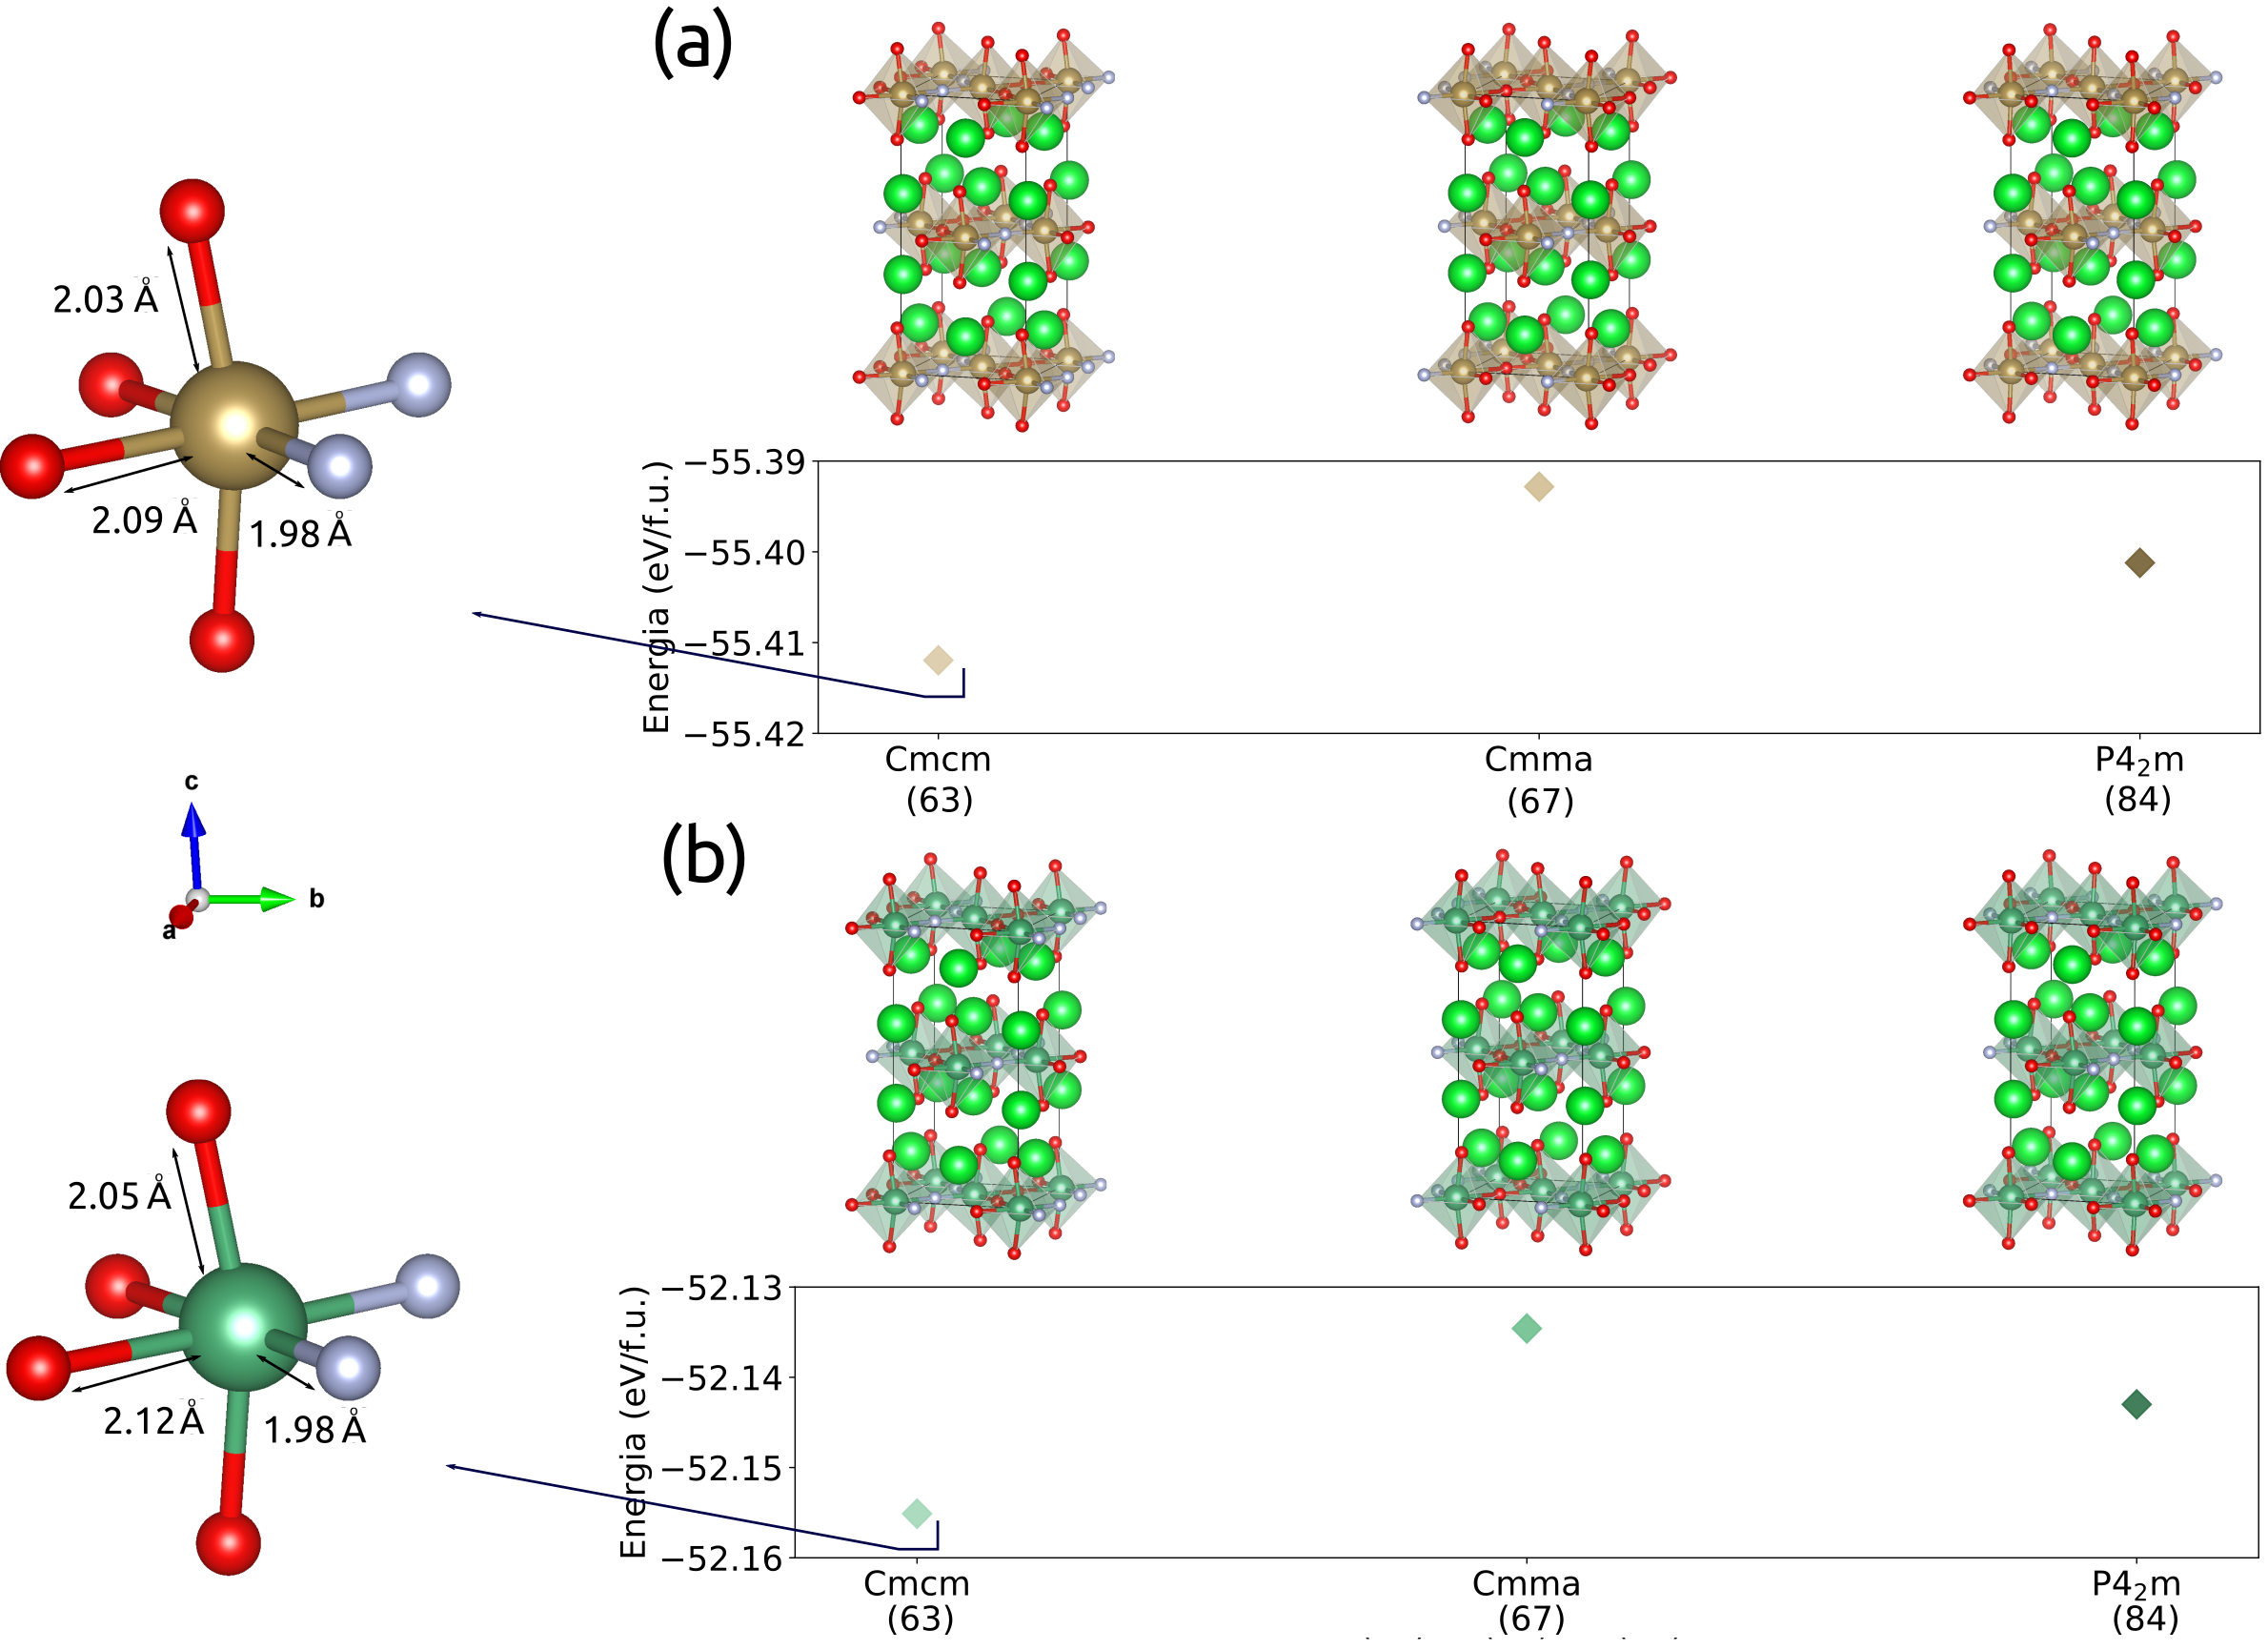
\includegraphics[width=\textwidth]{Figs/cis_energy_Ta.png}
    \caption{Energía estructural en relación a la simetría de grupo espacial de la configuración \textsc{rp}\emph{cis} (a) $Sr_{2}TaO_{3}N$ y (b) $Sr_{2}NbO_{3}N$.}
    \label{Fig. rp_cis}
\end{figure}

Las estructuras de mínima energía tienen simetría de grupo espacial $Cmcm(63)$ con un valor de $-55.41 eV$ y $-52.16 eV$ para $Sr_{2}TaO_{3}N$ y  $Sr_{2}NbO_{3}N$, respectivamente. Esta configuración favorable con ordenamiento aniónico \emph{cis} se sitúa sobre el plano y alterna capa a capa la orientación del ordenamiento, así como se reporta en la literatura \cite{Yang2011}.  Esta fase resulta ser la de mas baja energía para la concentración $x=1.0$, es decir, es mas estable que la configuración \emph{trans} con una diferencia de energía de $0.261 eV$ y $0.295  eV$ para $Sr_{2}TaO_{3}N$ y  $Sr_{2}NbO_{3}N$, respectivamente. Los parámetros de red de la configuración ($63$)-$Sr_{2}TaO_{3}N$ son $a=5.76750 \si{\angstrom}$, $b=5.84364 \si{\angstrom}$ y $c=12.44960 \si{\angstrom}$, $\alpha=\beta=\gamma=90^{\circ}$, y volumen $419.591059 \si{\angstrom}^{3}$,  lo parámetros de red de la configuración ($63$)-$Sr_{2}NbO_{3}N$ son $a=5.76750\si{\angstrom}$, $b=5.84364 \si{\angstrom}$ y $c=12.44960 \si{\angstrom}$, $\alpha=\beta=\gamma=90^{\circ}$, y volumen $419.591059  \si{\angstrom}^{3}$. Estos parámetro son de una supercelda creada para este ordenamiento aniónico. Comparando estos parámetro de red con las estructuras de óxidos puros, el parámetro en \emph{'a'} aumenta $\sim0.04  \si{\angstrom}$, siendo esta la dirección del enlace $(Ta,Nb)-N$, es decir la dirección del orden aniónico \emph{trans}, mientras que en la dirección \emph{'b'}, el parámetro de red disminuye $\sim0.01 \si{\angstrom}$.

La distancia de los enlaces $(Ta,Nb)-O$ en los sitios axiales se mantienen para ambos compuestos, entre $2.03  \si{\angstrom}$ y $2.05  \si{\angstrom}$, pero en los sitios ecuatoriales el enlace $(Ta,Nb)-O$ aumenta a $2,09  \si{\angstrom}$ y $2.12  \si{\angstrom}$ para $Sr_{2}TaO_{3}N$ y  $Sr_{2}NbO_{3}N$, respectivamente. Esto debido al desplazamiento sobre el plano del metal de transición $(Ta,Nb)$ en dirección [110] hacia el nitrógeno, ya que el enlace $(Ta,Nb)-N$ es de $1.98  \si{\angstrom}$ para ambos compuestos. El hecho de que el desplazamiento del metal de transición haya surgido, da un indicio de una posible fase ferroeléctrica en estas estructuras con ordenamiento aniónico \emph{cis}, ya que este fenómeno se da en materiales no centro-simétricos \cite{Cohen1992Oxides}.

%Las estructuras derivadas con orden de aniones \emph{trans} en el plano de aniones ecuatoriales son generalmente desfavorables porque tener aniones con dureza de Pearson similar uno al lado del otro maximiza la hibridación $\pi$ en los enlaces B-X. Por esta razón, la gran mayoría de oxifluoruros y oxinitruros exhiben unidades heterolépticas cis y fac, aunque estudios recientes han demostrado que la cepa puede inducir el orden de aniones trans \cite{Harada2019}. 





%Por lo tanto, para obtener una estructura polar que pueda exhibir ferroelectricidad o piroelectricidad, parecería esencial encontrar una ruta hacia una estructura trans ordenada. Una posible ruta para estabilizar un orden trans sería aprovechar la combinación de celosías epitaxiales en arquitecturas de película delgada para orientar los enlaces largos Ta-N perpendiculares al sustrato. \cite{Page2007LocalTheory}

%in dieléctrico SrT aO 2 N, el refinamiento de la estructura cristalina sugirió el orden de rango O / N y la inclinación local de octaedros cis-T aO 4 N 2,\cite{Masubuchi2013SynthesisCeramics}





%Esto es una consecuencia de la alta estabilidad del enlace metal-oxígeno que hace que la síntesis de compuestos de sustitución de aniones requiera el uso de métodos menos sencillos. \cite{Fuertes2012ChemistryPerovskites}









%La sustitución de O 2  por N 3  induce la sustitución cruzada de M 2+ por M 3+ o la formación de aniones vacantes, para mantener la neutralidad de carga [4] \cite{Masubuchi2013SynthesisCeramics}

%En la fase Ruddlesden-Popper, el átomo de niobio ($Nb$) muestra un estado de oxidación de $4+$ que no es estable en el aire a altas temperaturas, pero al sustituir un átomo de oxígeno por un átomo de nitrógeno en cada bloque de perovskita, pasaría de una oxidación de $Nb^{4+}$ a la más estable $Nb^{5+}$ como ocurre en la perovskita $SrNbO_{2}N$\cite{Tobias2004}. Además, debido a las similitudes en electronegatividad, polarizabilidad, radio iónico y número de coordinación entre el oxígeno y el nitrógeno, se permite la formación de estos tipos estructurales, así como la sustitución mutua de ambos aniones sobre los mismos sitios cristalográficos\cite{Tobias2004}.\\


